
%************************************************
\chapter{Evolución de codificadores JPEG}\label{ch:resultados_evolucion}
%************************************************

En \ref{ch:evolucion} se dio una breve introducción al cómputo evolutivo y a su
\emph{ ``taxonomía" }. Se concluyó que este proyecto entra dentro de la
clasificación de programación genética, ya que podemos ver las tablas de
cuantificación como genotipos y los codificadores resultantes como genotipos.
Para tener una base sobre la cual discutir los detalles de implementación, se
discutió como funciona el algoritmo: La población inicial, la función de
selección y el criterio de finalización.

% ============================================================
\section{Correctud y Conjunto de prueba} \label{sec:testset}
% ============================================================

El proyecto está dividió en tres partes: TinyJPEG, la implementación de JPEG
con compresión \emph{baseline} basada en la especificación \cite{jpeg-spec};
DummyJPEG, la versión modificada de JPEG que sirve para tener una función de
selección paralelizable, que tiene implementaciones paralelas para CPU y GPU; y
finalmente, el proyecto completo, llamado \emph{gp\_encoder}, que consta de un
algoritmo evolutivo descrito en \ref{ch:evolucion}, que utiliza DummyJPEG en su
función de selección y emite el resultado usando TinyJPEG.

La biblioteca TinyJPEG, a partir de ser lanzada como código libre, consiguió
una base de usuarios usándola en aplicaciones que van desde tareas escolares
hasta proyectos de investigación. Durante un año ha sido pulida mientras se han
encontrado problemas con distintos decodificadores.

El proyecto \emph{gp\_encoder} tiene la ventaja de contar con el uso al que ha
sido sometido TinyJPEG para asegurarse que se tiene una base sólida. Aunque la
implementación OpenCL no ha tenido pruebas fuera de las imágenes que se han
utilizado a lo largo del desarrollo, hasta la fecha no ha habido problemas

% ============================================================

% ============================================================
\section{Convergencia}
% ============================================================

Recordando la ecuación que usamos para nuestra función de seleccion:

\begin{equation}
f(T) = \frac{e(T)}{e(T_0)} + \alpha \Big(1 + \frac{s(T)}{s(T_0)}\Big)
\end{equation}\label{eq:fitness-repeated}

Se desea obtener la cota mínima.

Se sabe que $e(T_0)$ es siempre menor o igual a $e(T)$, ya que $T_0$ es la
tabla de cuantificación que consiste solo de valores 1, que denominamos
\emph{tabla unitaria}, que resulta en lo más cercano en JPEG con compresión
\emph{baseline} a una compresión sin pérdida. Por lo tanto, el primer parámetro
de la ecuación está en $[1, \infty)$.

De manera análoga, el tamaño de la imágen resultante al comprimir con la tabla
unitaria es el mayor posible. Entonces, el término $\frac{s(T)}{s(T_0)} \in (0,
1]$. Se encontró que un buen valor de $\alpha$ para conseguir imágenes de alta
calidad es 2. Por lo tanto, el segundo término de la ecuación $f(T)$ está en
$(2, 4]$

En base a esto, se concluye que para la función de selección, con una tabla de
cuantificación arbitraria, el mínimo valor posible es 3.

En esta sección se incluyen las gráficas de convergencia para las cuatro
imágenes de referencia, \ref{img:plot-diego}, \ref{img:plot-ghost},
\ref{img:plot-klay}, \ref{img:plot-pluto}.

Todas las figuras mostradas están normalizadas a 50 generaciones con un rango
de evaluación de la función de selección entre 3.5 y 5. Se usa una gráfica de
línea para mostrar el valor de la función de selección para los individuos más
aptos y se utilizan puntos para los peores individuos de cada generación. Se
usan puntos porque comúnmente ocurre que en alguna generación, el individuo
menos apto tenga un valor de selección mucho mayor a 5. Esto produce gráficas
con picos, que se quieren evitar. El caso común, sin embargo, es que los
individuos menos aptos también tienden a un punto de convergencia mientras la
evolución avanza.

Cabe notar que la gráfica para la imagen "Pluto" muestra que hubo una
convergencia en un relativamente pequeño número de generaciones. Para ver lo
que pasaba, se cambió la tasa de mutación:cruza de 0.5 a 0.8, resultando en la
figura \ref{fig:plot-pluto2}. Esto resulta en una gráfica
\emph{``escalonada"}, mostrando una evolución de 57 generaciones que produce una
tabla con valor de selección similar al del resultado original. Fue consistente
el encontrar que cualquier distribución distinta a 50/50 producía peores
resultados.

\begin{figure}[h]
    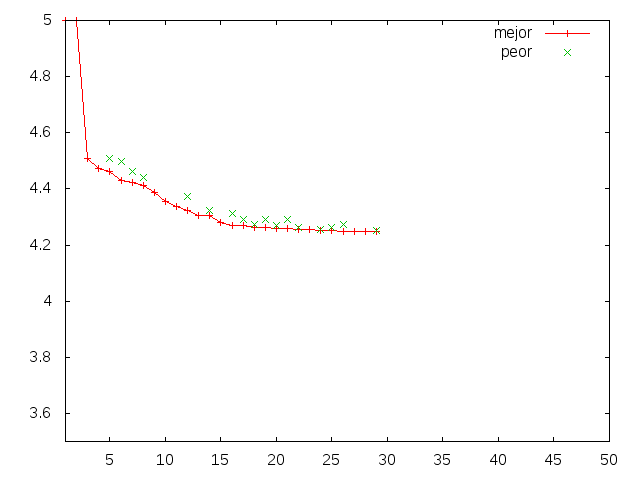
\includegraphics[width=1.0\textwidth]{plot_diego}
    \caption{Convergencia para imagen ``Diego"}
    \label{img:plot-diego}
\end{figure}

\begin{figure}[h]
    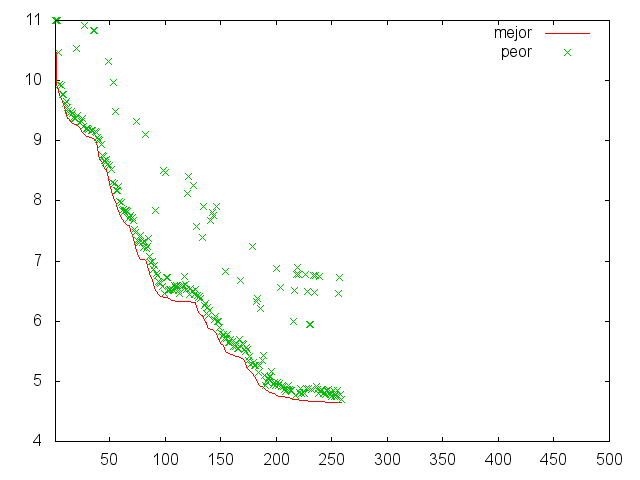
\includegraphics[width=1.0\textwidth]{plot_ghost}
    \caption{Convergencia para imagen ``Ghost"}
    \label{img:plot-ghost}
\end{figure}

\begin{figure}[h]
    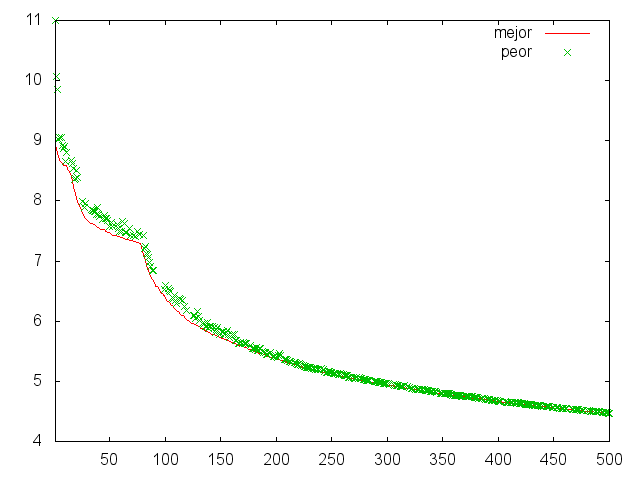
\includegraphics[width=1.0\textwidth]{plot_klay}
    \caption{Convergencia para imagen ``Klay"}
    \label{img:plot-klay}
\end{figure}

\begin{figure}[h]
    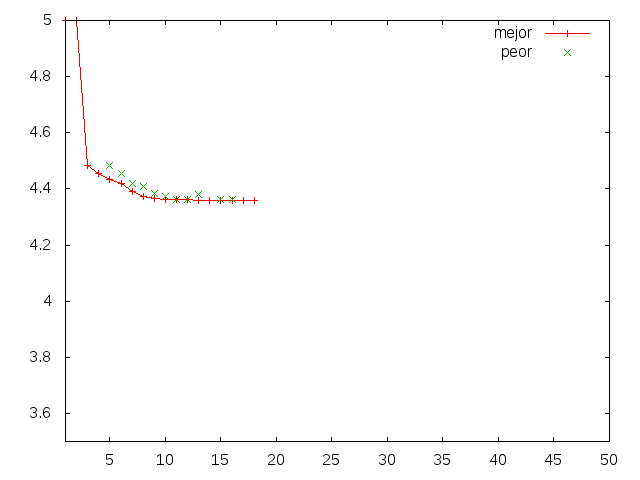
\includegraphics[width=1.0\textwidth]{plot_pluto}
    \caption{Convergencia para imagen ``Pluto"}
    \label{img:plot-pluto}
\end{figure}

\begin{figure}
    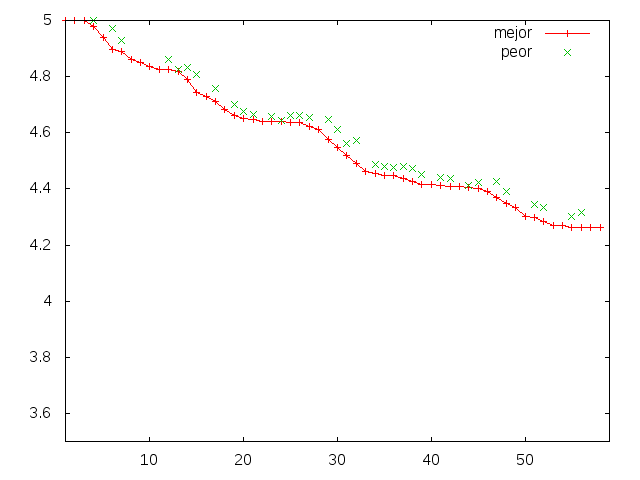
\includegraphics[width=1.0\textwidth]{plot_pluto_tweak}
    \caption{Convergencia para imagen Pluto con una tasa de mutación a cruza diferente}
    \label{img:plot-pluto2}
\end{figure}

% ============================================================
\section{Comparación de desempeño}
% ============================================================

La figura \ref{fig:perf_table} en esta sección es una copia de la que se
introdujo en el capítulo \ref{ch:implementacion}. La tabla muestra el desempeño
de gp\_encoder en sus diferentes modalidades: CPU (single-thread y multi-thread)
y GPU (OpenCL).

\begin{figure}[h]
    \begin{tabular}{ |l c c c c r| }
        \hline
        Nombre &  Un Thread & Múltiples Threads & GPU & Speedup MT & Speedup GPU \\
        \hline
        Diego & 10.796s & 5.210s & 1.391s  & 2.072X & 7.76X \\
        Ghost & 13.706s & 6.607s & 1.760s  & 2.257X & 7.78X \\
        Klay & 40.526s & 22.279s & 4.785s  & 1.819X & 8.46X \\%, 4.65
        Plutón & 558.83s & 204.120s & 13.940s & 2.73X & 40.08X \\ % 14.64
        \hline
    \end{tabular}
    \caption{Tabla de desempeño para gp\_encoder}
    \label{fig:perf_table}
\end{figure}


%TODO Tabla de tamaño para cada imagen. TinyJPEG calida máxima, media y con la tabla generada por DummyJPEG

